\subsection{Wasserstoff (1€/kg) - Szenarionummer 12}\label{chap_kenngrößen_s_12}

\subsubsection{Kenngrößen Ausgangssituation}
\captionof{table}{\label{table_12_kenngrößen_ausgangsszenario_infrastrukturkilometer} Kenngrößen Ausgangszenario genutzte Infrastruktur jeweils für \acrshort{spnv}, \acrshort{spfv} und \acrshort{sgv} sowie insgesamt}
\begin{center}
	\begin{tabularx}{\textwidth}{l | X | X | X} & Infrastruktur & Infrastruktur (nicht elektrifiziert) & Anteil nicht elektrifizierte Infrastruktur \\
	\hline
	\acrshort{sgv} & \SI{11211}{\km} & \SI{1152}{\km} & \num{10.28} \% \\
	\acrshort{spfv} & \SI{12989}{\km} & \SI{908}{\km} & \num{6.99} \% \\
	\acrshort{spnv} & \SI{22806}{\km} & \SI{10037}{\km} & \num{44.01} \% \\
	\hline
	Insgesamt & \SI{28739}{\km} & \SI{10191}{\km} & \\
	\end{tabularx}
\end{center}
\hspace{2em}

Hinweis: Länge der Infrastruktur weicht von bekannter Länge der Infrastruktur ab, da z.T. parallele Strecken aufgrund des Routing-Algorithmus nicht mitgerechnet werden können.

\captionof{table}{\label{table_12_kenngrößen_ausgangsszenario_betriebskilometer} Kenngrößen Ausgangszenario Zugkilometer jeweils für \acrshort{spnv}, \acrshort{spfv} und \acrshort{sgv} sowie insgesamt}
\begin{center}
	\begin{tabularx}{\textwidth}{l | X | X | X} & Zugkilometer gesamt (Tag) & Zugkilometer nicht elektrisch (Tag) & Anteil nicht elektrische Betriebslänge \\
	\hline
	\acrshort{sgv} & \SI{1395.49}{Tsd. \km} & \SI{59.916}{Tsd. \km} & \num{4.29}  \% \\
	\acrshort{spfv} & \SI{985.608}{Tsd. \km} & \SI{29.964}{Tsd. \km} & \num{3.04} \% \\
	\acrshort{spnv} & \SI{2272.498}{Tsd. \km} & \SI{712.496}{Tsd. \km} & \num{31.35} \% \\
	\hline
	Insgesamt & \SI{4653.596}{Tsd. \km} & \SI{802.376}{Tsd. \km} & \\
	\end{tabularx}
\end{center}


\subsubsection{Kenngrößen Szenario}
\captionof{table}{\label{table_12_kenngrößen_scenario} Basiskenngrößen Szenario 12}
\begin{center}
	\begin{tabularx}{\textwidth}{l | r } Kenngröße & Wert \\
	\hline
	Anzahl Untersuchungsgebiete & \num{155} \\
	Summe Streckenkilometer & \SI{10191}{\km} \\
	Summe Zugkilometer (Tag) & \SI{802.376}{Tsd. \km} \\
	\ce{CO2}-Jahresbilanz Ausgangssituation & \SI{2264868}{\tonne} \ce{CO2} \\
	\ce{CO2}-Jahresbilanz Szenario 12 & \SI{85150}{\tonne} \ce{CO2}\\
	\end{tabularx}
\end{center}

\subsubsection{Kenngrößen Untersuchungsgebiete}
\captionof{table}{\label{table_12_kenngrößen_untersuchungsgebiete} Anzahl Untersuchungsgebiete sowie Kilometer nach Traktion Szenario 12}
\begin{center}
	\begin{tabularx}{\textwidth}{X | r | r | r} Traktion & Anzahl & Kilometer Infrastruktur & Zugkilometer (Tag) \\
	\hline
            electrification & \num{46} &  \SI{1270}{\km} & \SI{288}{Tsd. \km}\\
            efuel & \num{0} &  \SI{0}{\km} & \SI{0}{Tsd. \km}\\
            battery & \num{84} &  \SI{4491}{\km} & \SI{379}{Tsd. \km}\\
            optimised electrification & \num{21} &  \SI{6548}{\km} & \SI{834}{Tsd. \km}\\
            diesel & \num{0} &  \SI{0}{\km} & \SI{0}{Tsd. \km}\\
            h2 & \num{4} &  \SI{1181}{\km} & \SI{103}{Tsd. \km}\\
            no calculated cost & \num{0} &  \SI{0}{\km} & \SI{0}{Tsd. \km}\\
    	\end{tabularx}
\end{center}

\captionof{table}{\label{table_12_kenngrößen_untersuchungsgebiete_no_optimised} Anzahl Untersuchungsgebiete sowie Kilometer nach Traktion (Optimierte Elektrifizierung aufgeteilt) Szenario 12}
\begin{center}
	\begin{tabularx}{\textwidth}{X | r | r | r} Traktion & Anzahl & Kilometer Infrastruktur & Zugkilometer (Tag) \\
	\hline
            electrification & \num{46} &  \SI{4537}{\km} & \SI{893}{Tsd. \km}\\
            efuel & \num{0} &  \SI{0}{\km} & \SI{0}{Tsd. \km}\\
            battery & \num{84} &  \SI{7772}{\km} & \SI{608}{Tsd. \km}\\
            diesel & \num{0} &  \SI{0}{\km} & \SI{0}{Tsd. \km}\\
            h2 & \num{4} &  \SI{1181}{\km} & \SI{103}{Tsd. \km}\\
            no calculated cost & \num{0} &  \SI{0}{\km} & \SI{0}{Tsd. \km}\\
    	\end{tabularx}
\end{center}
In dieser Tabelle wurden die Infrastrukturkilometer der Untersuchungsgebiete, bei denen die optimierte Elektrifizierung am wirtschaftlichsten war, auf die Traktionen Elektrifizierung und Batterie aufgeteilt (je nachdem, bei welchem Teiluntersuchungsgebiet welche Traktion am wirtschaftlichsten war)

\subsubsection{Kenngrößen Kosten}

\captionof{table}{\label{table_12_kenngrößen_investition_cost_by_traction} Investitionsvolumen sowie Betriebskosten (Barwert Preisstand 2016) Szenario 12}
\begin{center}
	\begin{tabularx}{\textwidth}{X | r | r} Traktion & Kosten Infrastruktur Barwert & Betriebskosten Barwert\\
	\hline
            electrification & \num{1390198} Tsd. € &  \num{7504444} Tsd. €\\
            efuel & \num{0} Tsd. € &  \num{0} Tsd. €\\
            battery & \num{237447} Tsd. € &  \num{8337521} Tsd. €\\
            optimised electrification & \num{4407128} Tsd. € &  \num{19391065} Tsd. €\\
            diesel & \num{0} Tsd. € &  \num{0} Tsd. €\\
            h2 & \num{205435} Tsd. € &  \num{2645885} Tsd. €\\
            no calculated cost & \num{0} Tsd. € &  \num{0} Tsd. €\\
    	\hline
		Summe & \num{6240208} Tsd. € & \num{37878915} Tsd. €
	\end{tabularx}
\end{center}

\begin{center}
	\begin{figure}[p]
	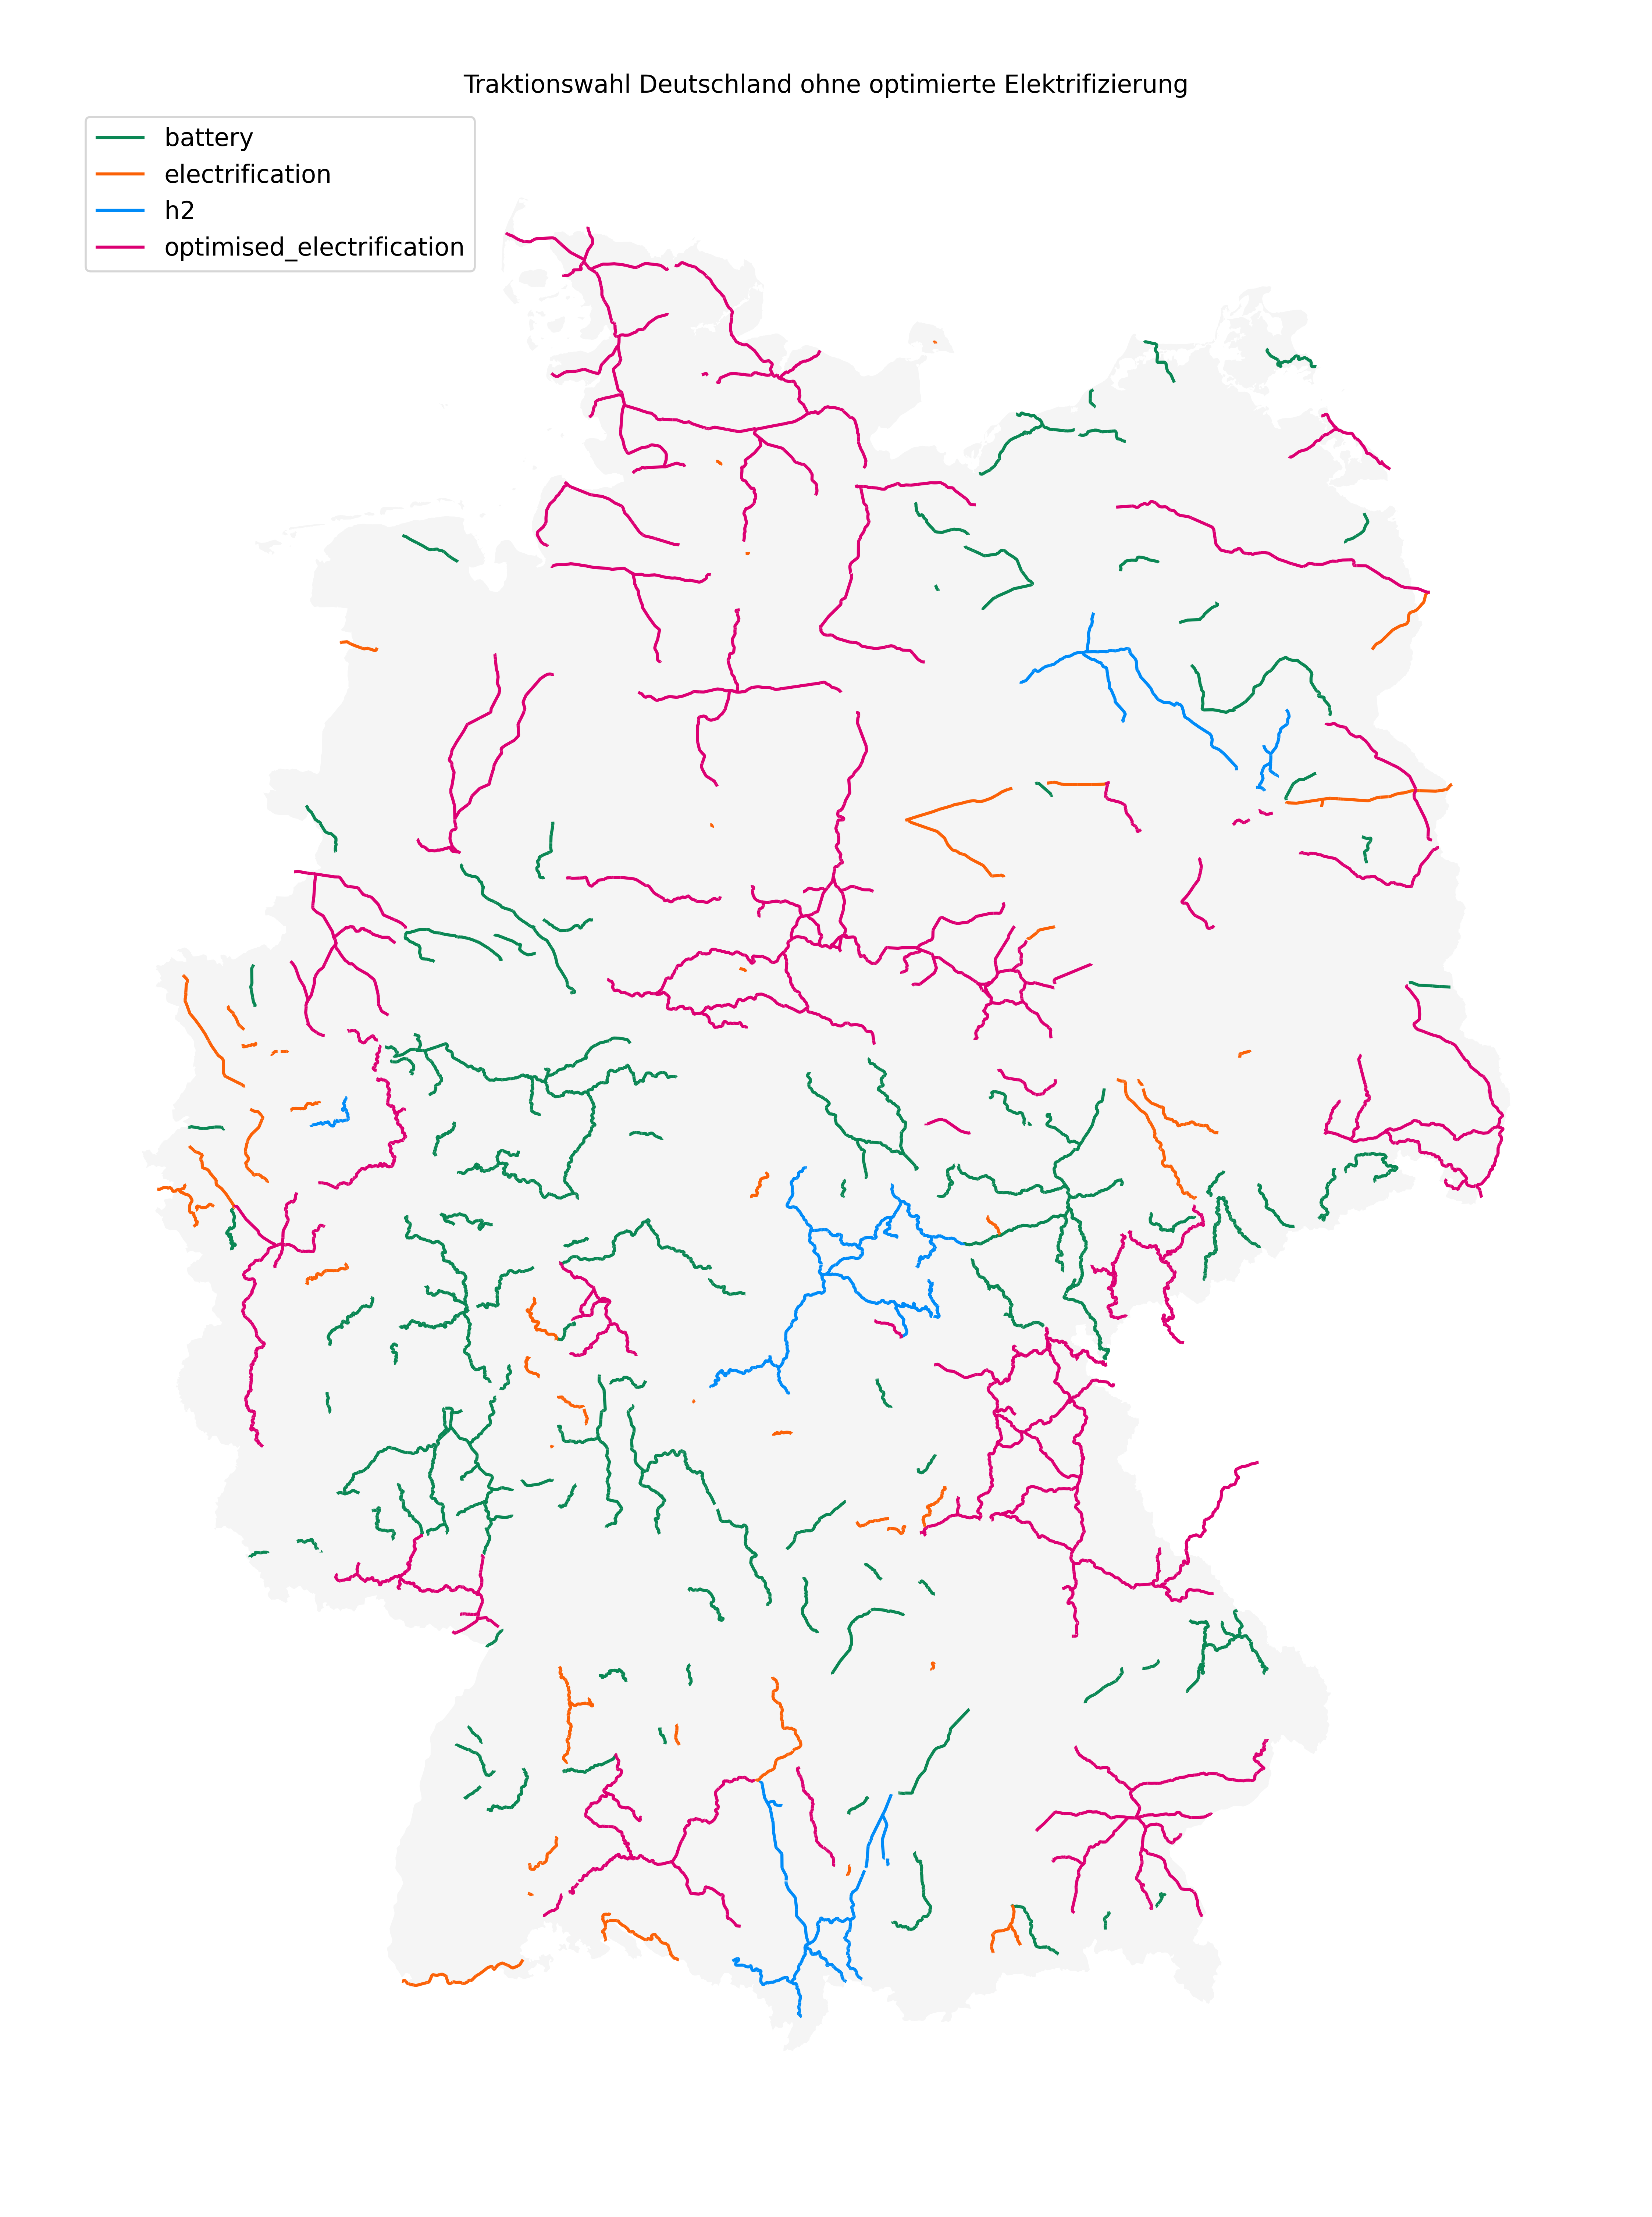
\includegraphics[height=0.8\textheight]{../report_scenarios/s_12/files/deutschland_map}
	\caption{\label{fig_s_12_d_map} Karte Deutschland bevorzugte Traktion Untersuchungsgebiete Szenario Wasserstoff (1€/kg)}
	\end{figure}
\end{center}

\subsubsection{Kenngrößen Güter-, Fern- und Nahverkehr}
\captionof{table}{\label{table_12_kenngrößen_sgv} Zugkilometer Güter-, Fern- und Nahverkehr Szenario 12 für Linien mit nicht elektrifizierten Abschnitten im Bezugsfall}
\begin{center}
\begin{tabularx}{\textwidth}{l|X|X|X|X|X} & Zkm elektrisch & Zkm Batterie & Zkm Wasserstoff & Zkm Diesel & Zkm E-Fuel \\
	\hline
	\uppercase{spnv} &
	\SI{658806}{\km} &
	\SI{590577}{\km} &
	\SI{102858}{\km} &
	\SI{0}{\km} &
	\SI{0}{\km} \\
	\uppercase{spfv} &
	\SI{103220}{\km} &
	\SI{17544}{\km} &
	\SI{0}{\km} &
	\SI{0}{\km} &
	\SI{0}{\km} \\
	\uppercase{sgv} &
	\SI{130993}{\km} &
	\SI{0}{\km} &
	\SI{0}{\km} &
	\SI{0}{\km} &
	\SI{0}{\km} \\
	\uppercase{all} &
	\SI{893019}{\km} &
	\SI{608120}{\km} &
	\SI{102858}{\km} &
	\SI{0}{\km} &
	\SI{0}{\km} \\
\end{tabularx}
\end{center}


%\begin{center}
%	\begin{tabularx}{\textwidth}{X | X } Kenngröße & Wert \\
%	\hline
%	Betriebsleistung \acrshort{sgv} (Linien mit Abschnitten ohne Oberleitung) & \SI{143.19073199999994}{Tsd. \km}
%	\end{tabularx}
%\end{center}